\documentclass{scrreprt}
\usepackage[utf8]{inputenc}
\usepackage{lmodern}
\usepackage{listings}
\usepackage{underscore}
\usepackage{graphicx}
\usepackage[margin=0.5in]{geometry}
\usepackage[bookmarks=true]{hyperref}
\hypersetup{
    bookmarks=false,    % show bookmarks bar?
    colorlinks=true,       % false: boxed links; true: colored links
    linkcolor=blue,       % color of internal links
    citecolor=black,       % color of links to bibliography
    filecolor=black,        % color of file links
    urlcolor=purple,        % color of external links
    linktoc=page            % only page is linked
}%
\def\myversion{1.0 }
\title{%
\flushleft
\rule{16cm}{5pt}\vskip1cm
\Huge{DESIGN SPECIFICATION}\\
for\\
Pok\'eSnowdown \\
\vspace{2cm}
\LARGE{Version \myversion\\}
\vspace{2cm}
Produced by Matthew Zang, Nicholas Cage, Chiraq Obama, 4Evar Young\\
\vfill
\rule{16cm}{5pt}
}
\renewcommand\thesection{\arabic{section}}
\renewcommand\thesubsection{\thesection.\arabic{subsection}}

\date{}
\usepackage{hyperref}
\begin{document}
\newgeometry{left=3cm,bottom=0.1cm}
\maketitle
\tableofcontents
\restoregeometry
\section{Update Log}

This log will hold all the updates/git pushes to our game, showing our current progress/what needs to be completed, etc...

\pagebreak 
\section{System Description}
\subsection{Core Vision}

Our plan for A6 is to create a Pok\'emon Showdown spinoff using \texttt{OCaml} using key concepts presented in class (concurrency, mutability, functional programming) as well as integrating functions of \texttt{OCaml} not presented in class, including producing a suitable GUI and server to aid in development of the game. To set us apart from Pok\'emon Showdown, we are incorporating a single-player story mode in the form of a "Tournament mode", as well as allowing for full 1-Player, 2-Player, and No-Player functionality (by developing an intelligent bot that can fully play the game).

\subsection{Key Features}
We hope to have the following implemented in our completed project:
\begin{enumerate}
	\item A fully functional GUI that allows the players to see the current state of the game. The GUI will most likely show the Pok\'emon but the attack animations might be too complex to complete. 
	\item All the current Pok\'emon will be included in the game, as well as items that are commonly used in competitive battling will also be included.
	\item Multiple game options. We are hoping to have the following modes.
		\begin{itemize}
			\item For 1-Player, we hope to incorporate three different modes. 
				\begin{enumerate}
					\item \textbf{Random Battles}: This is the same game mode as commonly found on Pok\'emon Showdown where teams are randomized. However, the player will be playing against the AI.
					\item \textbf{Tournament mode}: This is the single player story mode that we plan on incorporating.
					\item \textbf{Preset Battles}: The player gets to create his own Pok\'emon team and play against AI that use pre-made Smogon team compositions.
				\end{enumerate}
			\item For 2-Player, we hope to have a single game mode.
				\begin{enumerate}
					\item \textbf{Friend Battles}: Players have the options of choosing a Random team or a Preset team to head into battle with their friend.
				\end{enumerate}
			\item Lastly, for No-Player, we hope to have a single game mode.
				\begin{enumerate}
					\item \textbf{SkyNet Battles}: Player has option of choosing the Pok\'emon team for two bots, and watch them as they face off.
				\end{enumerate}
		\end{itemize}
	\item We wish to provide a Pok\'emon team editor that allows a player to choose Pok\'emon and movesets. This team is saved and can be loaded up for future use. These teams will be used in the game modes described above.
	\item We wish to integrate mustic into our game based upon the game mode as well as the current battle status.
	\item We want to include an interactive story mode/dialogue that will describe the underlying storyline in our Tournament mode. 
	\item We will have to include concurrency for two player battling, meaning that there will have to be a server to respond to player requests as well as the GUI. 
\end{enumerate}

\subsection{Narrative Description}
	This game will be an upgraded version of Pok\'emon Showdown, suitable and to the scale for a small console video game. It will have the main aspects of Pok\'emon Showdown including random battles between two players, as well as premade team battles between two players and a fully functional Pok\'emon team editor. However, it will also include single player capabilities, such as random battling or premade battling against an AI. The AI must be able to battle effectively and use advanced Pok\'emon techniques in the battle. In addition to this, there will be a Tournament mode which is essentially a story mode. The player has to play against several bots before proceeding to the final boss. This means that bots should have different levels of intelligence in order for this game mode to be challenging. 
\section{Architecture}
	We are aiming to produced a pipe and filter architecture. We were initially going to produce a client-server architecture with a game server keeping track of the current game state and updating the GUI will allowing clients (players) to send messages to the server to retrieve information and request actions; however, we realized that creating a server would make it hard to implement all the other features we wanted to implemented (since none of us knew what creating a server entailed). Instead of having a client-server architecture that allowed for two players to do concurrent battling, we realized that a pipelined architecture where each player would take turns choosing a move would work just as well. The input from the user will be passed along a pipeline and transforms the data into output. This is sufficient enough for the turn based Pok\'emon game. 
	
	However, in addition to the pipe and filter architecture (in relation to the game flow), we have some aspects of Shared Data Architecture. The Game and the GUI use the shared data architecture to communicate by reading and writing to the shared data. The C\&C diagram is provided below. The pipeline flow is shown from left to right, while the shared data architecture is shown extending downwards from Game Controller. 
	
	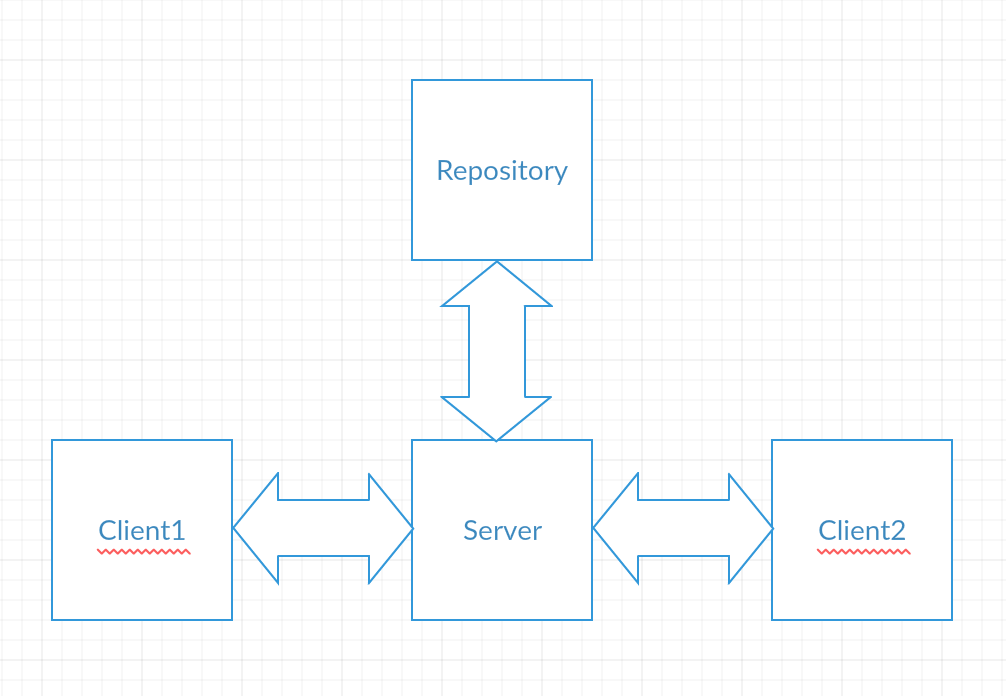
\includegraphics[scale=0.75]{C&C.png}

\section{System Design}
\subsection{Important Modules}

\begin{enumerate}
	\item \textbf{Game}: This is the game controller. It is mainly involved in handling the GUI and passing control to the battle controller when a battle occurs/is set up.
	\item \textbf{Gui}: The Gui is used to diplay the current state of the game. There are two main phases in the Gui, the menu screens and the battle scenes. The Gui will either communicate with the game controller when the menu screens are being displayed or communicate with the battle controller when a battle is occuring.
	\item \textbf{Info}: The Info module contains all the data types that are needed/shared between the module. It essentially contains everything the other modules need to use to communicate with one another and helps in avoiding circular dependencies. All data types needed for the game will be declared here.
	\item \textbf{BattleController}: This battle controller module is called by the game controller when a battle is taking place. During this time, the battle controller handles all the game mechanics and updates the Gui. The game controller waits for the battle to end before resuming control.
	\item \textbf{DataLoader}: This module is involved in loading the data from the json files. For example, functions in this method will be called to convert a string containing the name of the Pok\'emon to something of type Pok\'emon (defined in the Info module).
	
\end{enumerate}

\subsection{Module Dependency Diagram}
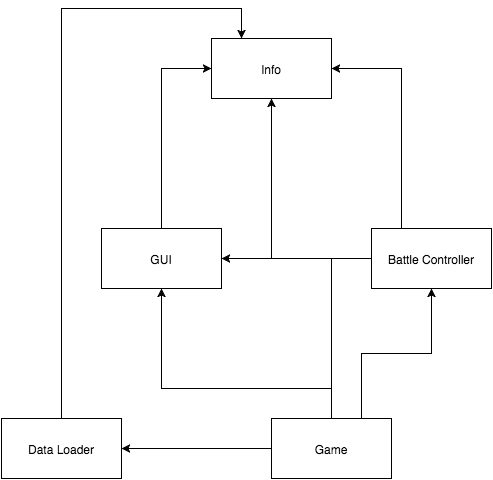
\includegraphics[scale=0.75]{MDD.png}

\section{Data}
%TODO Fill in internal data
\subsection{Internal Data}
We plan on having json files to represent all the Pok\'emon, moves, abilities, etc... Since json files aren't readily available online with all the Pok\'emon data, we wrote scripts to fetch the data from databases and convert them to a json format. To load the data, we are most likely going to use the Yojson module, similar to A3. 

%TODO Fill in communication
\subsection{Communication}
In order to let the GUI communicate with the Game without the use of a server, we came up with a method of communication through Ivar references. When Game initializes the GUI we make Game pass in as an argument an Ivar reference. Game and GUI communicate by emptying and filling the Ivar. When Game is ready to handle another input, Game resets the Ivar by creating a new one. GUI then fills in the Ivar when it gets some input. Thus, Game and GUI can communicate without creating any circular dependency within modules. The Ivar is filled with some variable that is of type \texttt{game\_state} defined in the Info module. 

%TODO Fill in data structures
\subsection{Data Structures}
To hold all the Pok\'emon data we will most likely be using some implementation of a dictionary. We are thinking of using a HashMap or the infamous Two-Three trees.

%TODO See if you can expand
\section{External Dependencies}

We will be using \texttt{Lablgtk2} to create the GUI and \texttt{Yojson} to parse json files. 

%TODO Fill in testing plan 
\section{Testing Plan}

% add other chapters and sections to suit
\end{document}